\documentclass[usenatbib,usegraphicx,letterpaper]{mn2e}
\usepackage[totalwidth=480pt,totalheight=680pt]{geometry}

\usepackage{amssymb}
\usepackage{epsfig}
\usepackage{amsmath}
\usepackage{color}
\usepackage[dvipsnames]{xcolor}
\usepackage{hyperref}
\usepackage{yfonts}

\usepackage{epsfig}  \usepackage{graphicx}   \usepackage{rotating}

%------- New commands

\newcommand{\lsim}{\lower0.6ex\vbox{\hbox{$ \buildrel{\textstyle <}\over{\sim}\ $}}}
\newcommand{\gsim}{\lower0.6ex\vbox{\hbox{$ \buildrel{\textstyle >}\over{\sim}\ $}}}
\newcommand{\beq}{\begin{equation}}
\newcommand{\eeq}{\end{equation}}


\newcommand{\mvir}{M_{\rm vir}}
\newcommand{\vmax}{v_{\rm max}}
\newcommand{\rvir}{R_{\rm vir}}
\newcommand{\ncen}{N_{\rm cen}}
\newcommand{\nsat}{N_{\rm sat}}
\newcommand{\ngal}{N_{\rm gal}}
\newcommand{\abias}{\mathcal{A}_{\rm bias}}

%%%%% less than approximate and all that

\def\gtsima{$\; \buildrel > \over \sim \;$}
\def\ltsima{$\; \buildrel < \over \sim \;$}
\def\prosima{$\; \buildrel \propto \over \sim \;$}
\def\gsim{\lower.7ex\hbox{\gtsima}}
\def\lsim{\lower.7ex\hbox{\ltsima}}
\def\simgt{\lower.7ex\hbox{\gtsima}}
\def\simlt{\lower.7ex\hbox{\ltsima}}
\def\simpr{\lower.7ex\hbox{\prosima}}
\def\la{\lsim}
\def\ga{\gsim}
\def\lta{\la}
\def\gta{\ga}

%------ Journals

\newcommand{\mnras}{Mon. Not. R. Astron. Soc.}
\newcommand{\apjl}{Astrophys. J. Lett.}
\newcommand{\aj}{Astron. J.}
\newcommand{\aap}{Astron. Astrophys.}
\newcommand{\araa}{Ann. Rev. Astron. Astroph.}
\newcommand{\apjs}{Astrophys. J. Suppl. Ser.}
\newcommand{\physrep}{Phys. Rep.}
\newcommand{\jcap}{JCAP}
\newcommand{\prd}{Phys. Rev. D}
\newcommand{\apj}{ApJ}

\newcommand{\wprp}{w_{\mathrm{p}}}
\newcommand{\rp}{r_{\mathrm{p}}}
\newcommand{\magr}{M_r}


\newcommand{\bit}{\begin{itemize}}
\newcommand{\eit}{\end{itemize}}
\newcommand{\ben}{\begin{enumerate}}
\newcommand{\een}{\end{enumerate}}


\bibliographystyle{mn2e}

%Title of paper---------------------------------------------------------


\title[Clustering Constraints on Assembly Bias]
{
Constraints on Assembly Bias from Galaxy Clustering. 
}

% Authors ------------------------------------------------------


\author[Zentner et al.]
{Andrew R. Zentner$^{1}$, Andrew P. Hearin$^{2}$, Frank C. van den Bosch$^{3},$ \newauthor
Antonio Villareal$^{1}$, Johannes U. Lange$^{3}$, P. Rogers Nelson$^{4}$\\ \\
$^1$Department of Physics and Astronomy \& Pittsburgh Particle Physics, Astrophysics, and Cosmology Center (PITT PACC),\\ University of Pittsburgh, Pittsburgh, PA 15260\\
$^2$Yale Center for Astronomy \& Astrophysics, Yale University, New Haven, CT\\
$^3$Department of Astronomy, Yale University, P.O. Box 208101, New Haven, CT\\
$^4$Paisley Park, Chanhassen, MN\\
}

\date{Today}

\pagerange{\pageref{firstpage}--\pageref{lastpage}} \pubyear{}

\newtheorem{theorem}{Theorem}[section]

\begin{document}

\maketitle
%----------------------------------------------------------------
%%%%%%%%%%%%%%%%%%%%%%%  A B S T R A C T %%%%%%%%%%%%%%%%%%%%%%%%%%%%%%
% ARZ: Important points:
% -supersedes previous analyses even for standard HOD.
% -cannot rule out assembly bias using galaxy clustering.
% -some samples favor assembly bias.
\begin{abstract}
We constrain the newly-introduced Decorated HOD model using SDSS DR7 measurements of projected galaxy clustering, $\wprp,$ and number density, $n_{\rm d},$ made from r-band luminosity-threshold samples. The Decorated HOD is a model for the galaxy--halo connection that augments the traditional Halo Occupation Distribution (HOD) by allowing for the possibility of {\em assembly bias}: galaxy luminosity may be correlated with dark matter halo properties besides virial mass $\mvir$ alone. We demonstrate that it is not possible to rule out assembly bias using DR7 measurements of $\wprp$ and $n_{\rm d}.$ Moreover, galaxy samples $\magr<-20, -20.5$ favor strong levels of central galaxy assembly bias: high-concentration halos are more likely to host a central galaxy relative to low-concentration halos of the same $\mvir.$ We rule out zero assembly bias with high significance for these samples. Satellite assembly bias only becomes significant for the faintest sample we study, $\magr<-19.$ We find no evidence for assembly bias in the $\magr<-21$ sample. Because the Decorated HOD subsumes the traditional HOD, and additionally because of errors made in the original analysis of these samples, our results differ from and supersede existing HOD constraints from low-redshift clustering measurements. 
\end{abstract} 

%---------------------------
\section{Introduction}
\label{section:introduction}
%---------------------------

For more than a decade, halo occupation modeling has been used to
interpret large-scale structure measurements and exploit these
measurements to constrain galaxy formation models and cosmology
\citep[e.g.,][]{yang03,tinker05,zehavi05a,
  porciani06,vdBosch07,Zheng07,conroy_wechsler09,yang09b,zehavi_etal11,guo_etal11b,
  wake_etal11,yang11a,yang12,leauthaud_etal12,rod_puebla12,tinker_etal13,cacciato_etal13,
  more_etal13,guo_etal14,zu_mandelbaum15b}. The key assumptions
underlying halo occupation modeling are: (1) all galaxies reside in
dark matter halos that are biased tracers of the density field; and
(2) galaxies occupy halos as a function of halo masses only. It is now
well known that halo bias depends upon halo properties other than mass
\citep[e.g.][]{gao_etal05,wechsler06,gao_white07,zentner07,dalal_etal08,lacerna11},
an effect called halo assembly bias. If galaxies occupy halos as a
function of properties other than halo mass, then standard halo
occupation methods will be subject to a systematic error due to galaxy
assembly bias. Several of us have previously shown that this error can
be significant in an analysis of galaxy clustering and can bias
inferences about many aspects of galaxy evolution
\citep{zentner_etal14}. Consequently, we have developed halo
occupation models that enable galaxies to occupy halos in a manner
that depends upon several halo properties \citep{hearin_etal16}.  See
also \citet{Yao_etalXX} for a similar approach. In this paper, we
revisit the interpretation of luminosity-dependent galaxy clustering
in the Sloan Digital Sky Survey (SDSS) Data Release 7 (DR7) data,
analyzed previously by \citet{zehavi_etal11}, in the context both
standard halo occupation models and these new models.

The ultimate goal of halo occupation modeling is to characterize the
galaxy-dark matter connection by constraining the probability
distribution $P(X_{\rm g}|Y_{\rm h})$. Here $X_{\rm g} = {x_1, x_2,
  ...x_n}$ is a set of $n$ galaxy properties, and $Y_{\rm h} = {y_1,
  y_2,...,y_m}$ a set of $m$ halo properties. Accurate knowledge of
this probability distribution yields invaluable insight to the
processes of galaxy formation, and allows one to make accurate
predictions for the clustering of galaxies as function of any property
$x_i$. Most halo occupation studies to date have restricted themselves
to only one halo property, namely halo mass.  This includes all Halo
Occupation Distribution (HOD) models, which aim to constrain
$P(N|\mvir)$, the probability that a halo of mass $M$ contains $N$
galaxies of some specified properties
\citep[e.g.,][]{kauffmann_etal97,jing98,benson01,berlind02}, and all
Conditional Luminosity Function (CLF) models, which aim to constrain
$\Phi(L|M)$, the luminosity (or stellar mass) function of galaxies in
haloes of mass $M$ \citep[e.g.,][]{yang03,vdBosch03a,cooray06}. The
HOD and CLF models are mainly used in combination with the halo model,
which describes the non-linear matter field in terms of halo building
blocks \citep[e.g.,][]{seljak00,cooray02}, to predict the clustering
of galaxies as function of luminosity or stellar mass.  Although
entirely analytical, and therefore fast, the downside of this method
is that it is extremely challenging to construct a model that is
accurate at the few percent level. The main issues are halo exclusion
\citep[see][]{smith_etal07,vdBosch13}, scale dependence of the
halo bias \citep[see][]{tinker05}, and the halo assembly bias mentioned
above.

These issues are trivially avoided by directly populating dark matter
haloes in numerical simulations with galaxies. This can be done using
either a parameterized model for the halo occupation statistics
\citep[e.g.,][]{Yang_etal04,moster10;behroozi10,behroozi13} or by
rank-order matching galaxy properties (i.e., luminosity or stellar
mass) to halo properties (i.e., halo mass). The latter method is known
as subhalo abundance matching (SHAM).  Although many SHAM studies use
halo mass as the halo property of choice
\citep[e.g.,][]{vale_ostriker04,vale_ostriker06,conroy07,conroy_wechsler09},
a number of studies have used alternative halo properties, such as the
maximum circular velocity, $\vmax$, or its peak value over the halo's
history, $V_{\rm peak}$
\citep[e.g.][]{tasitsiomi_etal04,conroy06,marin_etal08,reddick_etal13}

Since, at fixed halo mass, $\vmax$ is correlated with halo
concentration, and thus with halo assembly time, the resulting
occupation models have assembly bias build in
\citep[see][]{Zentner_etal14}; i.e., at fixed halo mass, galaxy
properties will be correlated with halo assembly
time. \citet{lehmann_etal15} took this one step further, and explored
SHAM models in which the halo property varies between $M$ and $\vmax$
via a continuously-valued parameter. Using SDSS clustering
measurements to constrain their model, they conclude that galaxy
luminosity reveals a significant dependence on halo
concentration. Since the latter is strongly correlated with halo
formation time \citep[e.g.,][]{wechsler02,zhao_etal09,ludlow_etal13},
their conclusions argue for non-zero assembly bias in the galaxy
population.

In addition to these studies that have focussed on constraining the
relation between a {\it primary} galaxy property (e.g., luminosity or
stellar mass) and a {\it primary} halo property (e.g., $M$ or
$\vmax$), there have also been a number of studies that relate
{\it secondary} galaxy properties (e.g., color or specific star
formation rate) to a {\it secondary} halo property (e.g., halo
formation time or concentration). The archetype of these model is the
`age-matching' model developed by \citet{HW13a}, in which galaxy color
is rank-order matched, at fixed stellar mass, to some quantity related
to the assembly history of the galaxy's (sub)halo.
Paranjape \etal 2015...


Another approach that 
This was taken one step further by Hearin ccc, who developed an
extension of SHAM, called age-matching. In age-matching a 




Our work is important for several reasons. Our work is a re-analysis
of the SDSS DR7 data that overcomes shortcomings of previous
analyses. In particular, we use direct population of galaxies in a
cosmological simulation so that delicate issues present in analytic
modeling, such as scale-dependent halo bias, are treated exactly.  The
simulation we use is based on the latest Planck cosmological
parameters, updating previous work. Furthermore, many important
differences between this work and the previous analysis by
\citet{zehavi_etal11} result from the fact that the Monte Carlo Markov
Chains used by Zehavi \etal where too small and had therefore not
converged (Z. Zheng \& I. Zehavi, Private Communication).  Therefore,
our analysis {\em supersedes previous analyses even in the case of
  standard halo occupation models}.

Furthermore, our work demonstrates explicitly that significant
assembly bias in $M_r$-selected samples from SDSS DR7 cannot be ruled
out based on a standard analysis of galaxy clustering only. In fact,
in agreement with \citet{lehmann_etal15}, we find that several samples
{\em favor galaxy assembly bias to a degree that is statistically
  significant}. As demonstrated by \citet{zentner_etal14}, this
conclusion could have important consequences for the interpretation of
both extant and forthcoming data.

Our paper is organized as follows. In Section~\ref{section:methods},
we discuss our implementation of halo occupation models and our
assumptions in our parameter inference analysis. We present results
for both standard halo occupation analysis and analysis in the context
of models with galaxy assembly bias in
Section~\ref{section:results}. We summarize our results and draw
conclusions in Section~\ref{section:conclusions}.

%---------------------------
\section{Methods}
\label{section:methods}
%---------------------------

%---------------------------
\subsection{Halotools Implementation of HOD Models}
\label{subsection:halotools}
%---------------------------

To generate predictions for galaxy clustering, we directly populate dark matter halos with mock galaxies using {\tt Halotools}. 
We explore halo occupation distribution models (HOD) models in this work 
\citep[e.g.][]{seljak00,ma_fry00,scoccimarro01a,berlind02}, though other 
techniques that can be used to interpret such data, such as the conditional luminosity function 
\citep[CLF, e.g.,][]{yang03,vdBosch13}, exist. In this section, we review the ``standard" HOD 
model used in the present work which assumes that there is no galaxy assembly bias. We refer to 
such a model as ``standard" because all HOD analyses of galaxy clustering to date have assumed no 
galaxy assembly bias. In the following section, we describe 
the Decorated HOD model described in \citet{hearin_etal16}. In both cases, we will only 
review the salient features of our methodology briefly; 
interested readers can always refer to {\tt halotools.readthedocs.io} and 
\citet{hearin_etal16} for further details. 

\subsubsection{Simulation}

All of our analyses are based on the Bolshioi-Planck simulation \citep{riebe_etal11}. 
Bolshoi-Planck was run with cosmological parameters based on \citet{planck13}, $\Omega_{\Lambda} = 0.693, \Omega_{\rm m} = 0.307, \Omega_{\rm b} = 0.048, h = 0.7, {\rm n_s}=0.96$ and $\sigma_8 = 0.82,$ within a cubic box 
$250$ ${\rm Mpc}/h$ on a side, requiring a particle mass of $m_{\rm p} = 1.35\times10^{8}M_{\odot}/h.$ 
Further information about the Bolshoi-Planck simulation is available at \url{https://www.cosmosim.org}. 

We use publicly available\footnote{\tt http://www.slac.stanford.edu/$\sim$behroozi/BPlanck\_Hlists} dark matter 
halo catalogs based on the {\tt ROCKSTAR} halo-finder \citep{behroozi_rockstar11} and {\tt CONSISTENT TREES} algorithm \citep{behroozi_trees13}. In particular, we use the {\tt halotools\_alpha\_version2} version of the $z=0$ snapshot 
of the {\tt `bolplanck'} catalog included with {\tt Halotools.} Halos in these catalogs are based on the virial radius 
density contrast given in \citet{bryan_norman98}. When populating this catalog with mock galaxies, we only use 
present-day host halos with a value of $M_{\rm peak}$ that exceeds $300$ particles. 


\subsubsection{Occupation statistics}

In standard HOD models, central galaxies and satellite galaxies are treated separately, so 
the model is specified by two probability distributions, one for each type of galaxy. 
The galaxy-halo connection is specified in terms of $P(\ncen|\mvir)$ and $P(\nsat|\mvir),$ 
the probability that a halo of mass $\mvir$ hosts $\ncen$ central and $\nsat$ satellite galaxies, 
respectively. $P(\ncen|\mvir)$ is typically a nearest-integer distribution, as a host halo has only 
either zero or one central galaxy. Consequently, the occupation statistics of central galaxies are 
specified by the first moment of $P(\ncen|\mvir)$, which we model as 
%
\begin{equation}
\label{eq:ncen}
\langle N_{\mathrm{cen}} \rangle(\mvir) =
        \frac{1}{2}\left( 1 +
        \mathrm{erf}\left( \frac{\log (\mvir) -
        \log (M_{\rm min})}{\sigma_{\log M}} \right) \right)
\end{equation}
%
For every host halo in the catalog we draw a random number from a uniform distribution $\mathcal{U}(0, 1);$ for a host halo of present-day virial mass $\mvir,$ a central galaxy is assigned to the halo if the associated random number is less than $\langle N_{\mathrm{cen}} \rangle(\mvir);$ halos with random values exceeding  $\langle N_{\mathrm{cen}} \rangle(\mvir)$ are left devoid of centrals. 
The parameter $\log (M_{\rm min})$ specifies the halo mass at which the halo has a 50\% probability of hosting a 
central galaxy, while the parameter $\sigma_{\log M}$ specifies the rate at which $\langle N_{\mathrm{cen}} \rangle (\mvir)$ 
transitions from zero to unity, with smaller values of $\sigma_{\log M}$ corresponding to a more rapid transition. 


We model the distribution $P(\nsat|\mvir)$ as a Poisson distribution with first moment given by a power law, 
%
\begin{equation}
\label{eq:nsat}
\langle N_{\rm sat}\rangle(\mvir) = \left( \frac{\mvir - M_0}{M_1} \right)^{\alpha}. 
\end{equation}
%
The parameter $M_0$ allows the power-law to be truncated more rapidly at low masses and we 
set $\langle N_{\rm sat}\rangle (\mvir) = 0$ for $\mvir < M_0$. 


The five parameters of the standard HOD models are varied in standard analyses are $\log (M_{\rm min})$, 
$\sigma_{\log M}$, $\alpha$, $\log (M_1)$, and $\log (M_0)$, though, as we show below, central galaxies usually 
outnumber satellite galaxies in by a factor of several, so $\log (M_{\rm min})$ and $\sigma_{\log M}$ usually 
vary along a narrow degeneracy that fixes the total galaxy number density to the observed value. There are 
many particular choices that can be made for the functional forms of $\langle N_{\rm cen}\rangle (\mvir)$ and 
$\langle N_{\rm sat}\rangle (\mvir)$. We have made choices that mimic the standard SDSS DR7 analysis of 
\citet{zehavi_etal11}, to expedite comparisons with their results.


\subsubsection{Galaxy profiles}

Central galaxies in the standard HOD models reside at the halo center, 
moving with the same velocity as the host halo peculiar velocity. We model 
the intra-halo spatial distribution of satellite galaxies to be located within $\rvir$ 
of the halo center, with a spherically symmetric NFW profile \citep{nfw97}. 
The concentration $c$ of each halo's satellite galaxy profile is taken to be 
the same as the concentration of the dark matter particles in the 
halo.\footnote{We set a maximum value of $c=25$ to the NFW concentration, 
because halos with very large values for the concentration tend to be poorly 
described by an NFW profile, for example due to a recent merger.}


We model the radial velocity distribution of satellite galaxies as a Gaussian with 
first moment equal to the host halo velocity and second moment equal to the 
solution to the isotropic Jeans equation for an NFW profile \citep{more09b}, 
\begin{equation}
\sigma^{2}_{r}(\tilde{r}|c) = V_{\rm vir}^{2}\frac{c^{2}\tilde{r}(1 + c\tilde{r})^{2}}{g(c)}\int_{c\tilde{r}}^{\infty}{\rm d}y\frac{g(y)}{y^{3}(1 + y)^{2}}, 
\end{equation}
where $\tilde{r} = r/\rvir,$ $g(x) = \rm{ln}(1+x) - x / (1+x),$ and $V_{\rm vir}^{2} = G\mvir/\rvir.$ 
We assume that velocities are isotropic, setting the peculiar velocities in each Cartesian direction 
according to random draws from the above radial velocity distribution. 

\subsubsection{Predictions for observables}

After populating a halo catalog with mock galaxies, we calculate the comoving number density of our mock galaxy sample as $n_{\rm g} = N_{\rm gal} / L_{\rm box}^3.$ We apply the distant-observer approximation and use the simulation z-axis as the line-of-sight direction, and the distance between points in the $xy$-plane to define the projected distance $\rp.$ We place mock galaxies into redshift-space by replacing each galaxy's $z$-coordinate with $z \rightarrow z + V_{\rm z}/H_0.$ We count pairs of points in each of our $\rp$ bins, rejecting pairs with $z-$distance exceeding $\pi_{\rm max}=60$ ${\rm Mpc/h.}$ We employ the \citet{landyszalay93} estimator to turn pair counts into a $\wprp$ prediction, as described in detail in {\tt halotools.readthedocs.io}. 

%---------------------------
\subsection{HOD with Assembly Bias: The Decorated HOD}
\label{subsection:decorated}
%---------------------------

In addition to the standard occupation statistics described in the previous section, 
in this paper we also use the decorated HOD formalism to connect galaxies t
o dark matter halos in a manner that has simultaneous dependence on both $\mvir$ and halo concentration. 
Briefly, we use Equations \ref{eq:ncen} and \ref{eq:nsat} as our ``baseline" first occupation moments. 
At fixed $\mvir,$ halos are divided into one of two categories, those of high- and low-concentration, 
depending on whether the concentration of the halo places it above or below the rank-order percentile 
$f_{\rm split},$ which we keep fixed to $f_{\rm split}=0.5$ throughout the paper for simplicity. 
High-concentration halos have a different first occupation moment relative to low-concentration 
halos of the same mass, $\langle\ngal|\mvir, c_{\rm high}\rangle \neq \langle\ngal|\mvir, c_{\rm low}\rangle.$ The difference between the first moment of high- and low-concentration halos is modulated by $\abias,$ the novel parameter of the decorated HOD governing assembly bias. Values of $\abias=\pm1$ correspond to the maximum strength of assembly bias allowable by the constraint that the model preserves the marginalized first moment, $\langle\ngal|\mvir\rangle;$ thus regardless of the value of $\abias,$ in the decorated HOD the marginalized first moment of centrals and satellites are {\em unchanged from the baseline value defined by Equations \ref{eq:ncen} and \ref{eq:nsat}}. 
Decorated HOD models all have the same HODs, when averaged over all halos at fixed mass, as standard HOD models. The only 
change in Decorated HOD models is whether or not an additional property also modulates halo occupation at fixed halo mass. A 
value of $\abias = 0$ indicates no galaxy assembly bias whatsoever. We refer the reader to \citet{hearin_etal16} for 
further details about the decorated HOD. 

In the present work, we fix our model to the simplest class of galaxy assembly bias models, though a recipe for 
generalizing to more complicated models can be found in \citet{hearin_etal16}. In particular, we split halos into 
two populations as specified in the previous paragraph. We then populate halos with satellite galaxies specified 
by an assembly bias parameter $-1 \le A_{\rm sat} \le 1$ and central galaxies with a distinct assembly bias 
parameter $-1 \le A_{\rm cen} \le 1$. These two additional parameters are varied in our analyses that include 
assembly bias, making the number of parameters that vary in these analyses seven. As we show below, 
these additional parameters are in many instances poorly constrained by clustering data of the quality of 
SDSS DR7 alone, so exploring more complex models of assembly bias does not yet seem justified.

%---------------------------
\subsection{Parameter Inference}
\label{subsection:mcmc}
%---------------------------

To infer parameters for the HOD and Decorated HOD models described in the previous subsections, 
we performed a Markov Chain Monte Carlo (MCMC) sampling of the posteriors using the 
affine-invariant ensemble sampler of \citet{goodman_weare10} as implemented in the 
{\tt emcee} software package \citep{foreman-mackey_etal13}. For most cases, we find that 
$\sim 3-10 \times 10^{6}$ samples are necessary in order for our chains to converge. 


%-------------------------------------------------------------------------------------------------------------------------------------------------
\begin{table}
\begin{center}
{\renewcommand{\arraystretch}{1.3}
\renewcommand{\tabcolsep}{0.2cm}
\begin{tabular}{l c}
\hline 
\hline
Parameter & Prior Interval\\ 
\hline
$\log (M_{\mathrm{min}})$ & [9.0,14.0] \\
$\sigma_{\log M}$ & [0.01,1.5] \\
$\log (M_0)$ & [9.0,14.0]\\
$\log (M_1)$ & [10.7,15.0]\\
$\alpha$ & [0.0,2.0]\\
$A_{\mathrm{cen}}$ & [-1.0,1.0]\\
$A_{\mathrm{sat}}$ & [-1.0,1.0]\\
\hline
\end{tabular}
\medskip
\caption{
Ranges for the priors used in the parameter inference. All prior distributions are uniform over the 
specified ranges.}
 }
 \label{table:priors}
 \end{center}
\end{table}
%--------------------------------------------------------------------------------------------------------------------------------


The most important detail of this analysis is the priors on the parameters. In all analyses 
discussed in this paper, we adopt priors that are uniform distributions over the intervals 
specified in Table~\ref{table:priors}. In the case of the assembly bias parameters 
$A_{\mathrm{cen}}$ and $A_{\mathrm{sat}}$, the priors represent physical 
boundaries. These parameters must satisfy $-1 \le A_{\mathrm{cen,sat}} \le 1$. 
Physical considerations require parameter $\sigma_{\log M} > 0$. All other 
priors have a negligible influence on the posterior aside from $\log M_0$. 
We find that $\log M_0$ is often very poorly constrained by clustering data.


%---------------------------
\section{Results}
\label{section:results}
%---------------------------

We have performed parameter inference analyses in order to infer the underlying HOD of 
galaxies from the projected galaxy two-point function $\wprp(\rp)$ as described in the preceding 
section. In this section, we describe the primary results of these analyses. Our marginalized 
one-dimensional parameter constraints are given in Table~\ref{table:parameters}.

%-------------------------
\subsection{Standard Analysis}
\label{subsection:standard}
%-------------------------

Prior to discussing our results using models that include assembly bias, we present 
results of standard HOD analyses that include no model for assembly bias. The results of 
the standard HOD analyses and all other analyses are shown in the form of marginalized 
constraints on individual parameters in Table~\ref{table:parameters}. We compare our parameter 
constraints to the standard HOD analysis performed by \citet{zehavi_etal11} in Table~\ref{table:parameters} 
as well. An example of the inferred posteriors for the HOD parameters is shown in Figure~\ref{fig:Mr20triangle}. 
The left-hand panels of Figure~\ref{fig:Mr19samples}, Figure~\ref{fig:Mr20samples}, and Figure~\ref{fig:Mr21samples} 
show the projected correlation function data along with predictions for $\wprp(\rp)$ from 50 randomly-selected 
models from the MCMC chains. Note that the significant covariance in the data makes it difficult to 
determine the quality of fit from visual inspection of these figures.


%--------------------------No AB Triangle Plot-----------------------------------------------------------------------------
\begin{figure*}
\begin{center}
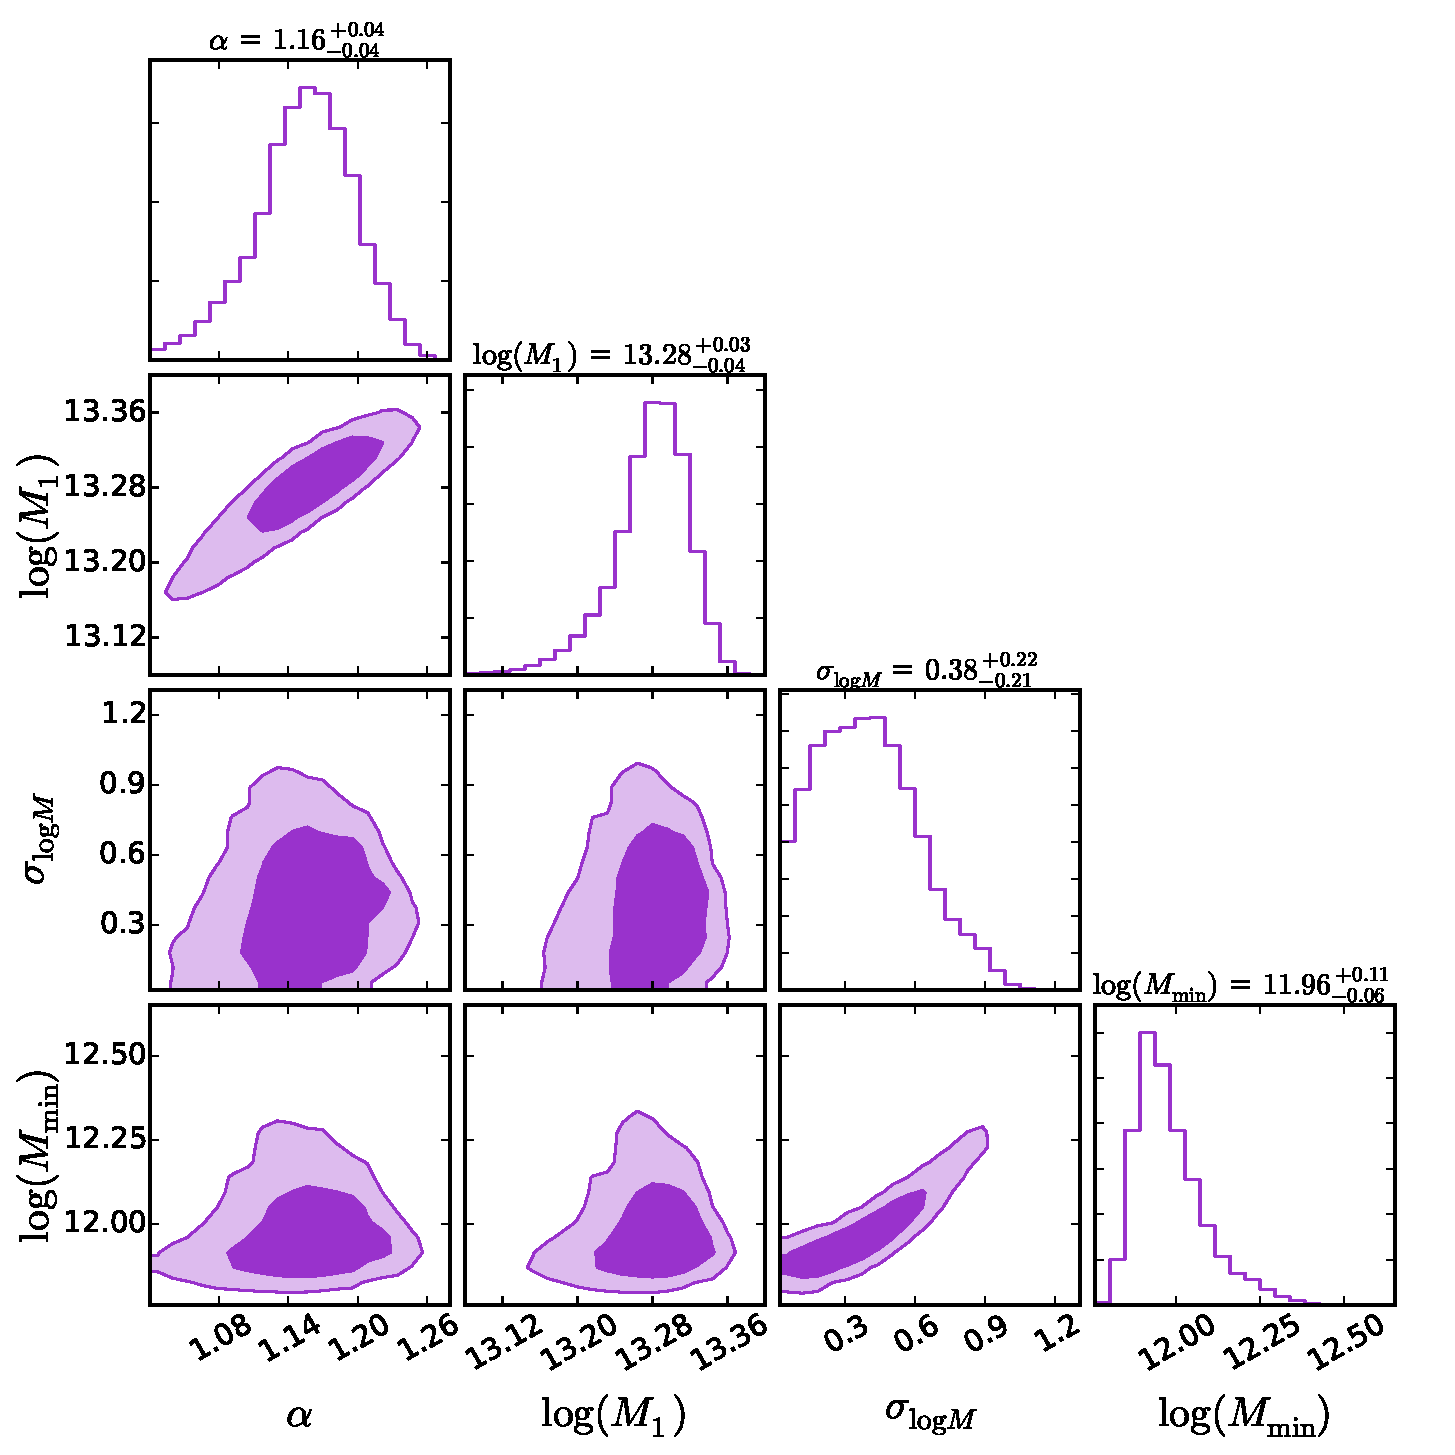
\includegraphics[width=15.0cm]{Mr20_covar_triangle_1.pdf}
\caption{
Two-dimensional marginalized constraints on HOD parameters inferred from 
standard HOD fits to $\wprp(\rp)$ data for the $M_r<-20$ sample. The HOD parameter 
$\log (M_0)$ is extremely poorly constrained by the $\wprp(\rp)$ data and has been 
omitted. The inner contours contain $68\%$ of the posterior probability while the 
outer contours contain $95\%$ of the probability. The panels along the diagonal 
show the one-dimensional, marginalized posteriors on each of these parameters. 
The values above each panel on the diagonal show the 
median value for the parameter in our chains along with the 
16$^{\rm th}$ and 84$^{\rm th}$ percentiles. 
}
\label{fig:Mr20triangle}
\end{center}
\end{figure*}
%----------------------------------------------------------------------------------------------------------------------------------

The inferred parameters from our standard analyses differ in several ways from the \citet{zehavi_etal11} 
analysis. Firstly, in our re-analysis of the projected clustering data, we generally find all mass scales to 
be slightly higher than in the work of \citet{zehavi_etal11}. This difference is largely due to the slightly 
different cosmologies adopted in this work. The most important difference 
are in the values of $\Omega_{\rm M}$, and $\sigma_8$.  
\citet{zehavi_etal11} assumed $\Omega_{\rm M}=0.25$ and $\sigma_8=0.8$, 
whereas in the present work, we use the BolshoiP simulation in which $\Omega_{\rm M}=0.307$ and $\sigma_8=0.82$. 
Slightly larger mass scales are necessary in an analysis with higher $\Omega_{\rm M}$ and $\sigma_8$ in order 
to maintain galaxy number densities with larger halo number densities.

 
%-------------------------------------------------------------------------------------------------------------------------------------------------
\begin{table*}
{\renewcommand{\arraystretch}{1.3}
\renewcommand{\tabcolsep}{0.2cm}
\begin{tabular}{l l c c c c c c c}
\hline 
\hline
Sample $M_r$ &  Authors & $\log (M_{\rm min})$ & $\sigma_{\log M}$ & $ \log (M_1)$ & $\alpha$ & $A_{\rm cen}$ & $A_{\rm sat}$ & $\chi^2/\mathrm{DoF}$\\ 
\hline
$-21$ & Zehavi+11 & $12.78 \pm 0.10$ & $0.68 \pm 0.15$ & $13.80 \pm 0.03$ & $1.15 \pm 0.06$ & $--$ & $--$ & 3.1\\
$-21$ & Zentner+16 & $12.92^{+0.07}_{-0.11}$ & $0.74^{+0.09}_{-0.16}$ & $13.93^{+0.04}_{-0.05}$ & $1.23^{+0.10}_{-0.12}$ & $--$ & $--$ & 1.59\\
$-21$ & Zentner+16 & $12.83^{+0.11}_{-0.09}$ & $0.60^{+0.15}_{-0.17}$ & $13.93^{+0.05}_{-0.08}$ & $1.16^{+0.12}_{-0.14}$ & $0.29^{+0.44}_{-0.35}$ & $0.08^{+0.49}_{-0.36}$ & 1.34 \vspace*{5pt}\\
%
$-20.5$ & Zehavi+11 & $12.14 \pm 0.03$ & $0.17 \pm 0.15$ & $13.44 \pm 0.03$ & $1.15 \pm 0.03$ & $--$ & $--$ & 2.7\\
$-20.5$ & Zentner+16 & $12.25^{+0.07}_{-0.03}$ & $0.23^{+0.17}_{-0.15}$ & $13.59^{+0.02}_{-0.02}$ & $1.20^{+0.04}_{-0.04}$ & $--$ & $--$ & 1.90\\
$-20.5$ & Zentner+16 & $12.32^{+0.13}_{-0.08}$ & $0.45^{+0.21}_{-0.25}$ & $13.59^{+0.04}_{-0.04}$ & $1.14^{+0.05}_{-0.06}$ & $>0.08 (90\%)$ & $0.22^{+0.40}_{-0.31}$ & 1.40 \vspace*{5pt}\\
%
$-20$ & Zehavi+11 & $11.83 \pm 0.03$ & $0.25 \pm 0.11$ & $13.08 \pm 0.03$ & $1.00 \pm 0.05$ & $--$ & $--$ & 2.1\\
$-20$ & Zentner+16 & $11.95^{+0.11}_{-0.6}$ & $0.37^{+0.23}_{-0.21}$ & $13.28^{+0.03}_{-0.04}$ & $1.16^{+0.04}_{-0.04}$ & $--$ & $--$ & 2.19\\
$-20$ & Zentner+16 & $12.23^{+0.33}_{-0.21}$ & $0.84^{+0.37}_{-0.31}$ & $13.20^{+0.06}_{-0.08}$ & $1.05^{+0.06}_{-0.08}$ & $ >0.28 (99\%) $ & $0.01^{+0.32}_{-0.26}$ & 1.16 \vspace*{5pt}\\
%$-20^d$ & Zentner+16 & $11.91^{+0.10}_{-0.03}$ & $0.26^{+0.25}_{-0.17}$ & $13.34^{+0.04}_{-0.05}$ & $1.25^{+0.05}_{-0.06}$ & $--$ & $--$ & 0.70 \\
%$-20^d$ & Zentner+16 & $12.00^{+0.29}_{-0.12}$ & $0.51^{+0.42}_{-0.32}$ & $13.31^{+0.06}_{-0.09}$ & $1.17^{+0.08}_{-0.09}$ & $0.76^{+0.18}_{-0.43}$ & $0.11^{+0.37}_{-0.34}$ & 0.30\vspace*{3pt}\\
$-19.5$ & Zehavi+11 & $11.57 \pm 0.04$ & $0.17 \pm 0.13$ & $12.87 \pm 0.03$ & $0.99 \pm 0.04$ & $--$ & $--$ & 1.00 \\
$-19.5$ & Zentner+16 & $11.76^{+0.33}_{-0.11}$ & $0.51^{+0.51}_{-0.29}$ & $13.05^{+0.04}_{-0.08}$ & $1.12^{+0.04}_{-0.07}$ & $--$ & $--$ & 1.24\\
$-19.5$ & Zentner+16 & $11.80^{+0.36}_{-0.16}$ & $0.63^{+0.53}_{-0.37}$ & $13.04^{+0.09}_{-0.12}$ & $1.06^{+0.07}_{-0.10}$ & $>-0.01 (84\%)$ & $>-0.16 (84\%)$ & 0.69 \vspace*{5pt}\\
%
$-19$ & Zehavi+11 & $11.45 \pm 0.04$ & $0.19 \pm 0.13$ & $12.64 \pm 0.04$ & $1.02 \pm 0.02$ & $--$ & $--$ & 1.8 \\
$-19$ & Zentner+16 & $11.72^{+0.33}_{-0.19}$ & $0.69^{+0.52}_{-0.46}$ & $12.78^{+0.04}_{-0.04}$ & $1.03^{+0.04}_{-0.04}$ & $--$ & $--$ & 2.77\\
$-19$ & Zentner+16 & $11.62^{+0.33}_{-0.13}$ & $0.53^{+0.57}_{-0.35}$ & $12.83^{+0.06}_{-0.07}$ & $1.02^{+0.04}_{-0.04}$ & $0.35^{+0.45}_{-0.66}$ & $>0.02 (84\%)$ & 2.01\\
%$-19^d$ & Zentner+16 & $11.87^{+0.17}_{-0.27}$ & $1.10^{+0.30}_{-0.52}$ & $12.84^{+0.17}_{-0.23}$ & $1.11^{+0.15}_{-0.15}$ & $--$ & $--$ & 2.30 \\
%$-19^d$ & Zentner+16 & $11.75^{+0.24}_{-0.27}$ & $0.94^{+0.41}_{-0.55}$ & $12.99^{+0.14}_{-0.18}$ & $1.17^{+0.14}_{-0.14}$ & $-0.17^{+0.50}_{-0.47}$ & $$ & 1.70\\
\hline
\end{tabular}
\medskip
\caption{
Results of standard HOD fits to SDSS DR7 $w_{\rm p}(r_{\rm p})$ as well as 
fits using a parameterized model of assembly bias. 
Assembly bias is quantified by the parameters $A_{\rm cen}$ ($A_{\rm sat}$) for central (satellite) galaxies. The secondary 
property that we assume to determine the galaxy HOD is halo concentration. $A_{\rm cen,sat}=0$ means that there is no 
assembly bias while $A_{\rm cen,sat}=1$ ($A_{\rm cen,sat}=-1$) means that galaxy abundance is maximally 
correlated (anticorrelated) with halo concentration at fixed $\mvir.$ Thus the $A_{\rm cen,sat}$ parameters span the range $[-1, 1].$ 
If the constraints on $A_{\rm cen}$ and $A_{\rm sat}$ are unspecified in the table, then the model used to interpret the data 
does not include assembly bias. In our analyses, quoted parameter values with errors correspond to the median 
value of the parameter and the 16$^{\rm th}$ and 84$^{\rm th}$ percentiles. In cases for which the posterior 
is monotonic within the physical parameter space, we show one-sided percentiles.
}
}
 \label{table:parameters}
\end{table*}
%---------------------------------------------------------------------------------------------------------------------------------


%----------------------------------------------------------------------------------------------------------------------------------
\begin{figure*}
\begin{center}
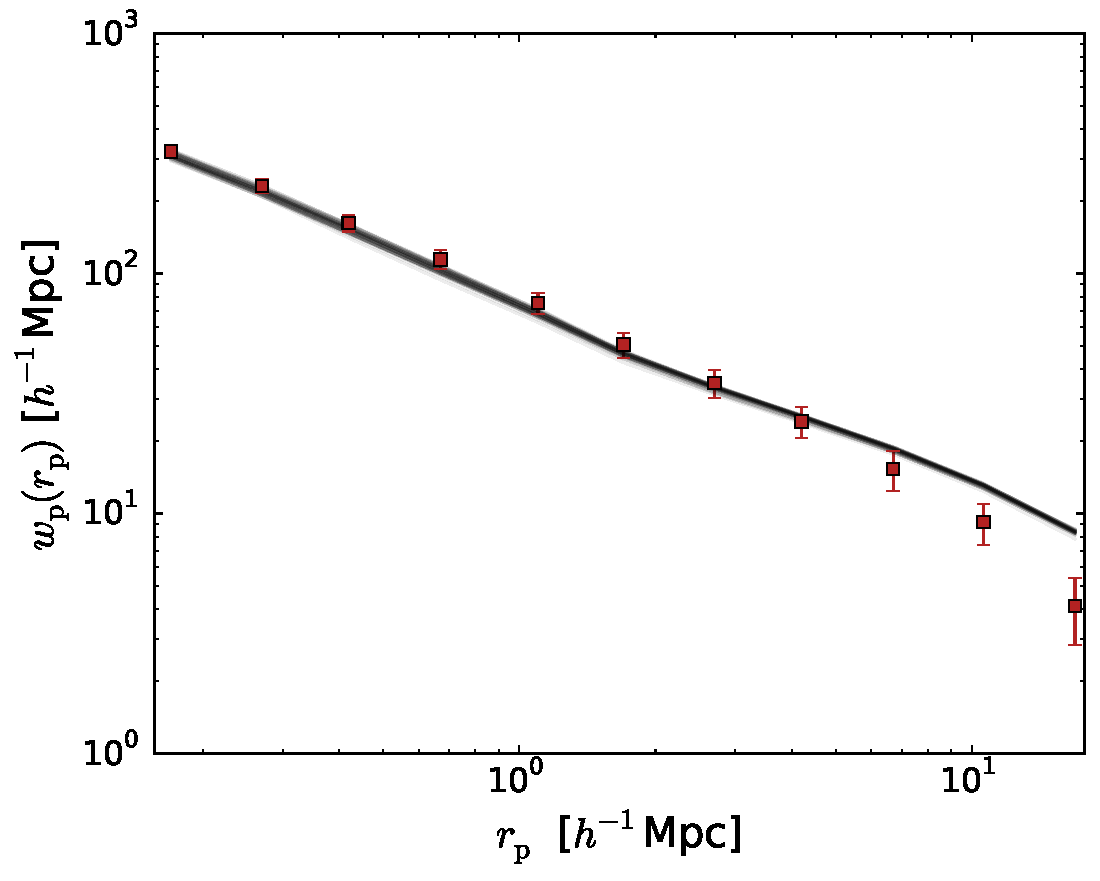
\includegraphics[width=8.3cm]{Mr19samples.pdf}
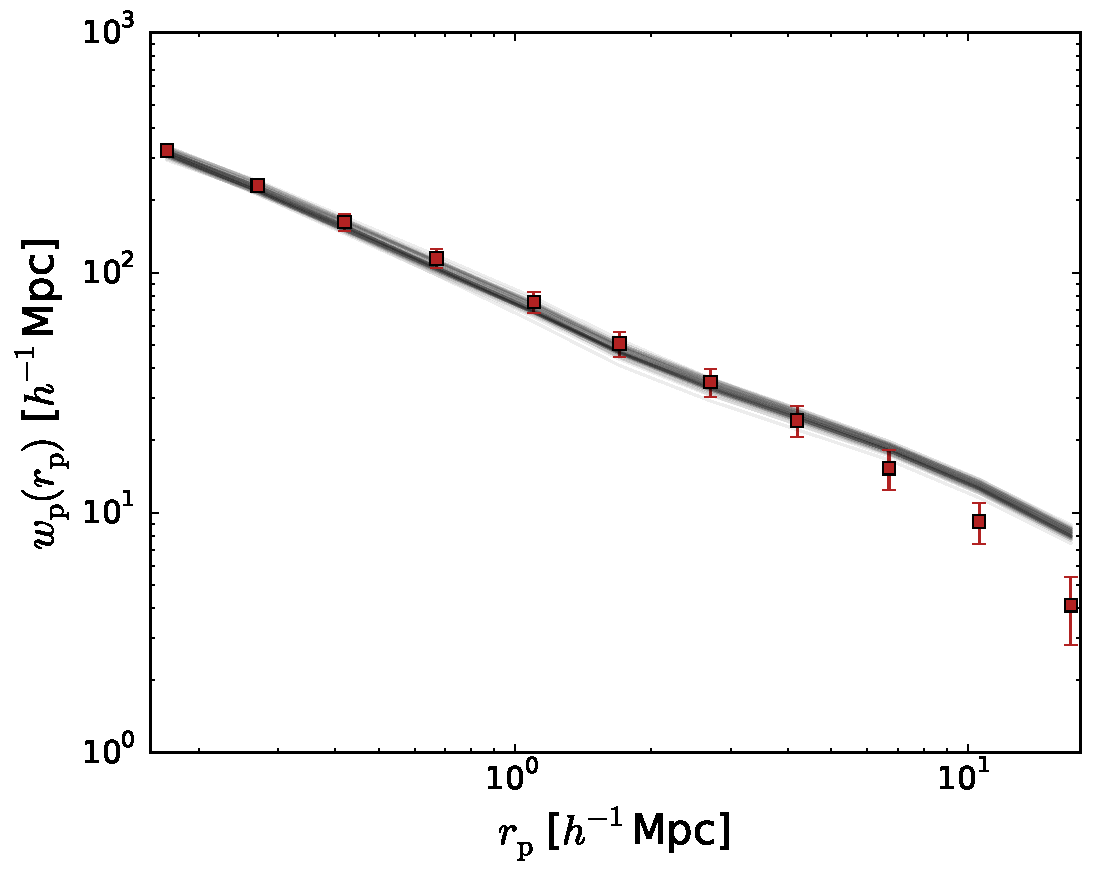
\includegraphics[width=8.3cm]{Mr19ABsamples.pdf}
\caption{
{\bf Left:} The $M_r<-19$ threshold sample projected correlation function with diagonal elements of 
covariance (points with errorbars). The grey lines are 25 randomly-selected HOD models that yield 
$\Delta \chi^2 <1$ compared to the best-fitting model. {\bf Right:} Same as the left panel but using a 
fit to a Decorated HOD model that contain parameters to describe the strength of assembly bias.
}
\label{fig:Mr19samples}
\end{center}
\end{figure*}
%---------------------------------------------------------------------------------------------------------------------------------


%---------------------------------------------------------------------------------------------------------------------------------
\begin{figure*}
\begin{center}
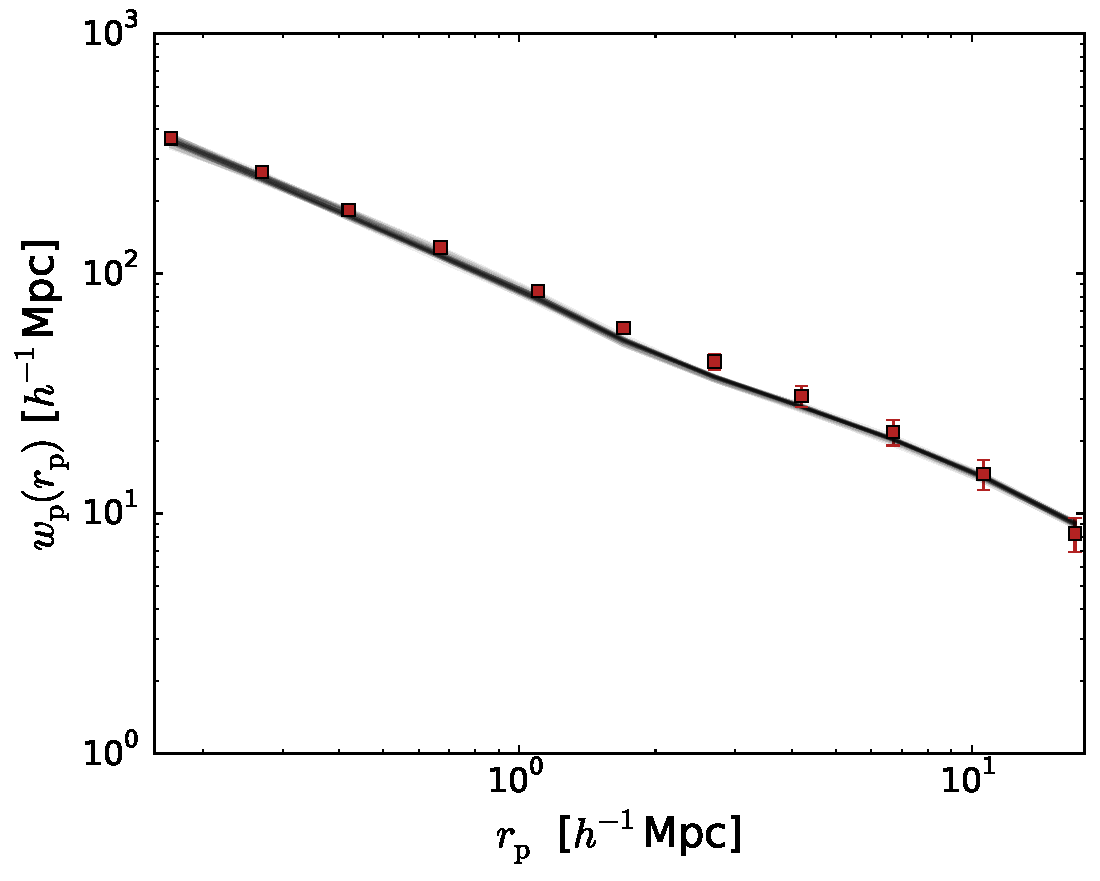
\includegraphics[width=8.3cm]{Mr20samples.pdf}
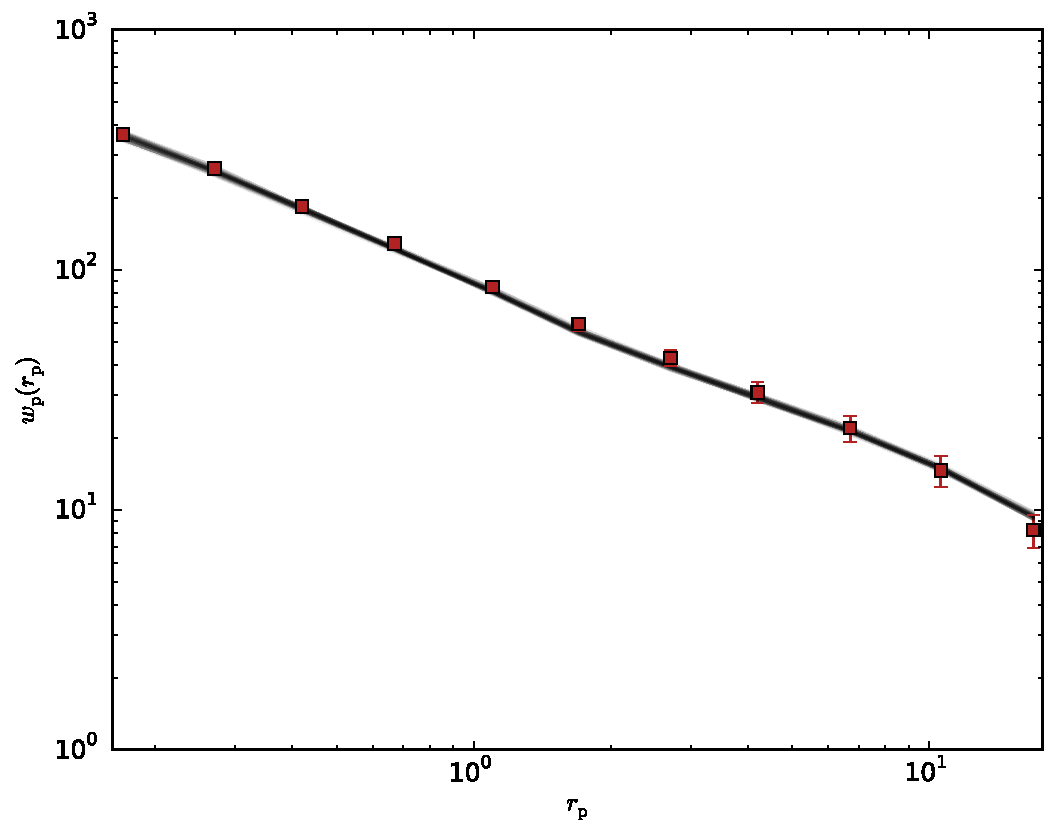
\includegraphics[width=8.3cm]{Mr20ABsamples.pdf}
\caption{
The same as Figure~\ref{fig:Mr19samples}, but for the $M_r<-20$ threshold sample.
}
\label{fig:Mr20samples}
\end{center}
\end{figure*}
%---------------------------------------------------------------------------------------------------------------------------------


%---------------------------------------------------------------------------------------------------------------------------------
\begin{figure*}
\begin{center}
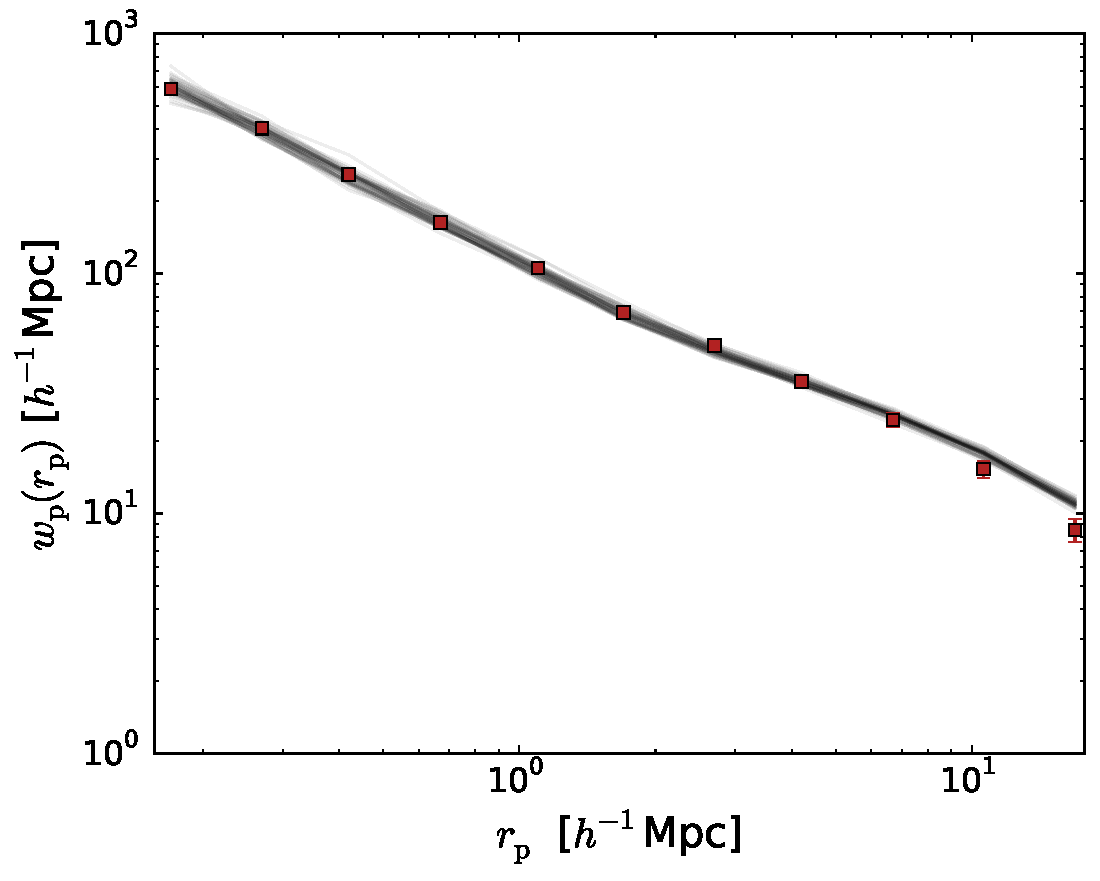
\includegraphics[width=8.3cm]{Mr21samples.pdf}
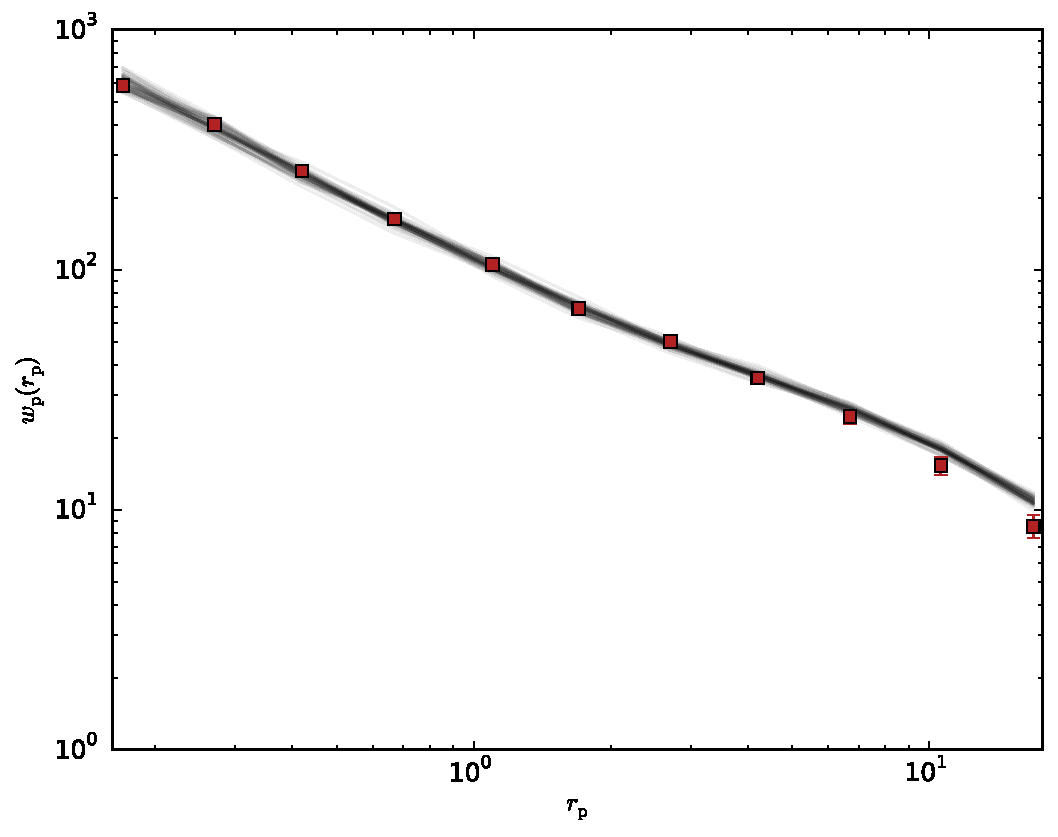
\includegraphics[width=8.3cm]{Mr21ABsamples.pdf}
\caption{
The same as Figure~\ref{fig:Mr19samples}, but for the $M_r<-21$ threshold sample.
}
\label{fig:Mr21samples}
\end{center}
\end{figure*}
%---------------------------------------------------------------------------------------------------------------------------------


A second noteworthy difference between the present work and that of
\citet{zehavi_etal11} is that we find many parameters to be notably
more poorly constrained. At the lower luminosity thresholds, for
example, we constrain $\log (M_{\rm min})$ and $\sigma_{\log M}$ with
several times lower precision than \citet{zehavi_etal11}. We do not
show our constraints on $\log (M_0)$ as they are very poor, with
1-sigma constraints $\gta 1$~dex for all samples. In several cases,
the constraint on $\log (M_0)$ is determined by the prior given in
Table~\ref{table:priors}. This is in stark contrast to several of the
results of \citet{zehavi_etal11}. For example, for the threshold
sample with $M_r < -19.5$ ($M_r < -20.5$), \citet{zehavi_etal11} quote
$\log (M_0) = 12.23 \pm 0.17$ ($12.35 \pm 0.24$), whereas we infer
$\log (M_0) = 11.38^{+0.95}_{-1.57}$
($11.19^{+0.89}_{-1.39}$). Examining the form of Eq.~(\ref{eq:nsat}),
it is sensible that the parameter $\log (M_0)$ should be unconstrained
at the lower end, because the value of $M_0$ does not alter the
predicted satellite number once $M_0 \ll M_1$. Therefore, it seems
likely that the tighter constraints quoted by \citet{zehavi_etal11}
must be an error.

Additionally, we have confirmed with a subset of the authors of \citet{zehavi_etal11} 
that the number of MCMC samples they included in their analysis was 
insufficient in a number of cases and that this can lead to a significant underestimation of the uncertainties 
on the inferred parameters, especially $\log (M_{\rm min})$ and $\sigma_{\log M}$ 
(Z. Zheng \& I. Zehavi, private communication). The analysis of \citet{zehavi_etal11} 
used $10^4$ samples, whereas we find several $\times 10^6$ samples are often necessary for convergence. 
Additionally, we have recreated qualitatively similar behavior by considering only small subsets of our 
full MCMC chains. Consequently, insufficient sampling of the posterior seems to be the likely resolution 
of the discrepancies between our work and that of \citet{zehavi_etal11}.

Two degeneracies are manifest in Fig.~\ref{fig:Mr20triangle} that are common to all of our 
analyses. The parameters $\log (M_1)$ and $\alpha$ are degenerate with each other and positively 
correlated. The parameter $M_1$ is the mass scale at which a halo has one satellite on 
average, and $\alpha$ is the power-law index describing the dependence of average satellite 
number on halo mass. Increasing $M_1$ {\em decreases} the number of satellites in massive halos 
by increasing the mass scale where the power law abundance becomes operative. An increase in $\alpha$ can partly 
compensate for an increase in $M_1$ by increasing the rate at which average satellite number 
grows with halo mass. 

As is evident in Figure~\ref{fig:Mr20triangle}, $\log (M_{\rm min})$ and $\sigma_{\log M}$ 
share a relatively narrow degeneracy as well. This degeneracy is largely induced by the 
measured number density of the sample. Increasing $\log (M_{\rm min})$ decreases galaxy 
number density, but this can be compensated by an increase in $\sigma_{\log M}$, which 
places galaxies in a fraction of the considerably more numerous halos with masses less 
than $M_{\rm min}$. The consequence is that $\log (M_{\rm min})$ and $\sigma_{\log M}$ are 
degenerate with each other such that most of the posterior probability lies in a narrow band 
along which $\log (M_{\rm min})$ and $\sigma_{\log M}$ are positively correlated, as shown in 
Fig.~\ref{fig:Mr20triangle}. In the following plots, we suppress the parameter $\sigma_{\log M}$,  
in order to increase the clarity of the plots, because the viable range of $\sigma_{\log M}$ is 
determined by this simple degeneracy with $\log (M_{\rm min})$. 

The results of this subsection demonstrate that we achieve reasonable fits to projected galaxy clustering 
data using direct HOD population of a high-resolution numerical simulation of structure formation. These results 
also update and supersede existing constraints in the literature in at least three respects. First, we work within the 
best-fit Planck cosmology. Second, we perform our parameter inference analysis using direct population of halos 
identified in a numerical simulation of cosmological structure formation (BolshioP). This greatly mitigates modeling 
uncertainties associated with nonlinear density field evolution, scale-dependent halo bias, halo exclusion, 
or other effects that have been difficult to incorporate into analytical halo models with high precision. Third, 
we have explored the posteriors of the parameters with significantly more samples (roughly two orders of magnitude), 
thereby mitigating errors on inferred parameters and their errors induced by insufficient sampling of the 
posterior.

%-------------------------
\subsection{Analysis with Decorated HOD}
\label{subsection:ab}
%-------------------------

We turn now to a discussion of our parameter inference analysis of projected galaxy clustering 
in Decorated HOD models that include a treatment of galaxy assembly bias. In this work, 
we consider only the simplest model of galaxy assembly bias, introducing only two new 
parameters, $A_{\rm cen}$ and $A_{\rm sat}$, that describe the strength of central galaxy 
and satellite galaxy assembly bias respectively. These parameters are limited to values 
of $-1 \le A_{\rm cen,sat} \le 1$, and $A_{\rm cen,sat}=0$ when there is no galaxy assembly bias. 
In this work, we use halo concentration as our secondary halo property, so $A_{\rm cen,sat}=1$ 
($A_{\rm cen,sat}=-1$) means that the mean number of galaxies per halo is maximally 
correlated (anti-correlated) with halo concentration. The model and its implementation 
in {\tt halotools} is discussed further in Section~\ref{subsection:decorated} above and 
in \citet{hearin_etal16}.

Examples of our fits are given in the right-hand panels of Figure~\ref{fig:Mr19samples}, 
Figure~\ref{fig:Mr20samples}, and Figure~\ref{fig:Mr21samples}. The general trend that 
can be gleaned from these figures is that introducing assembly bias improves the ability 
of the predicted two-point functions to match the measured two-point functions across the 
transition form the one-halo (highly nonlinear) to two-halo (nearly linear) regimes near $\rp \sim 2\, h^{-1}{\mathrm{Mpc}}$. 
This is most apparent for the $M_r < -20$ threshold sample shown in Fig.~\ref{fig:Mr20samples}. 
Visually, these differences appear to be small; however, Table~\ref{table:parameters} shows that 
they are statistically important.

The one-dimensional marginalized constraints on all parameters from these analyses 
are given in the lowest row of each luminosity threshold grouping in Table~\ref{table:parameters}. 
In cases where the posterior on a parameter is monotonic within the physical parameter 
range, we quote an upper or lower limit on the parameter. One- and two-dimensional 
visualizations of the posteriors from our analysis are shown in Figure~\ref{fig:Mr19ABtriangle}, 
Figure~\ref{fig:Mr20ABtriangle}, and Figure~\ref{fig:Mr21ABtriangle}. 


%------------------------------------------------------------------------------------------------
\begin{figure*}
\begin{center}
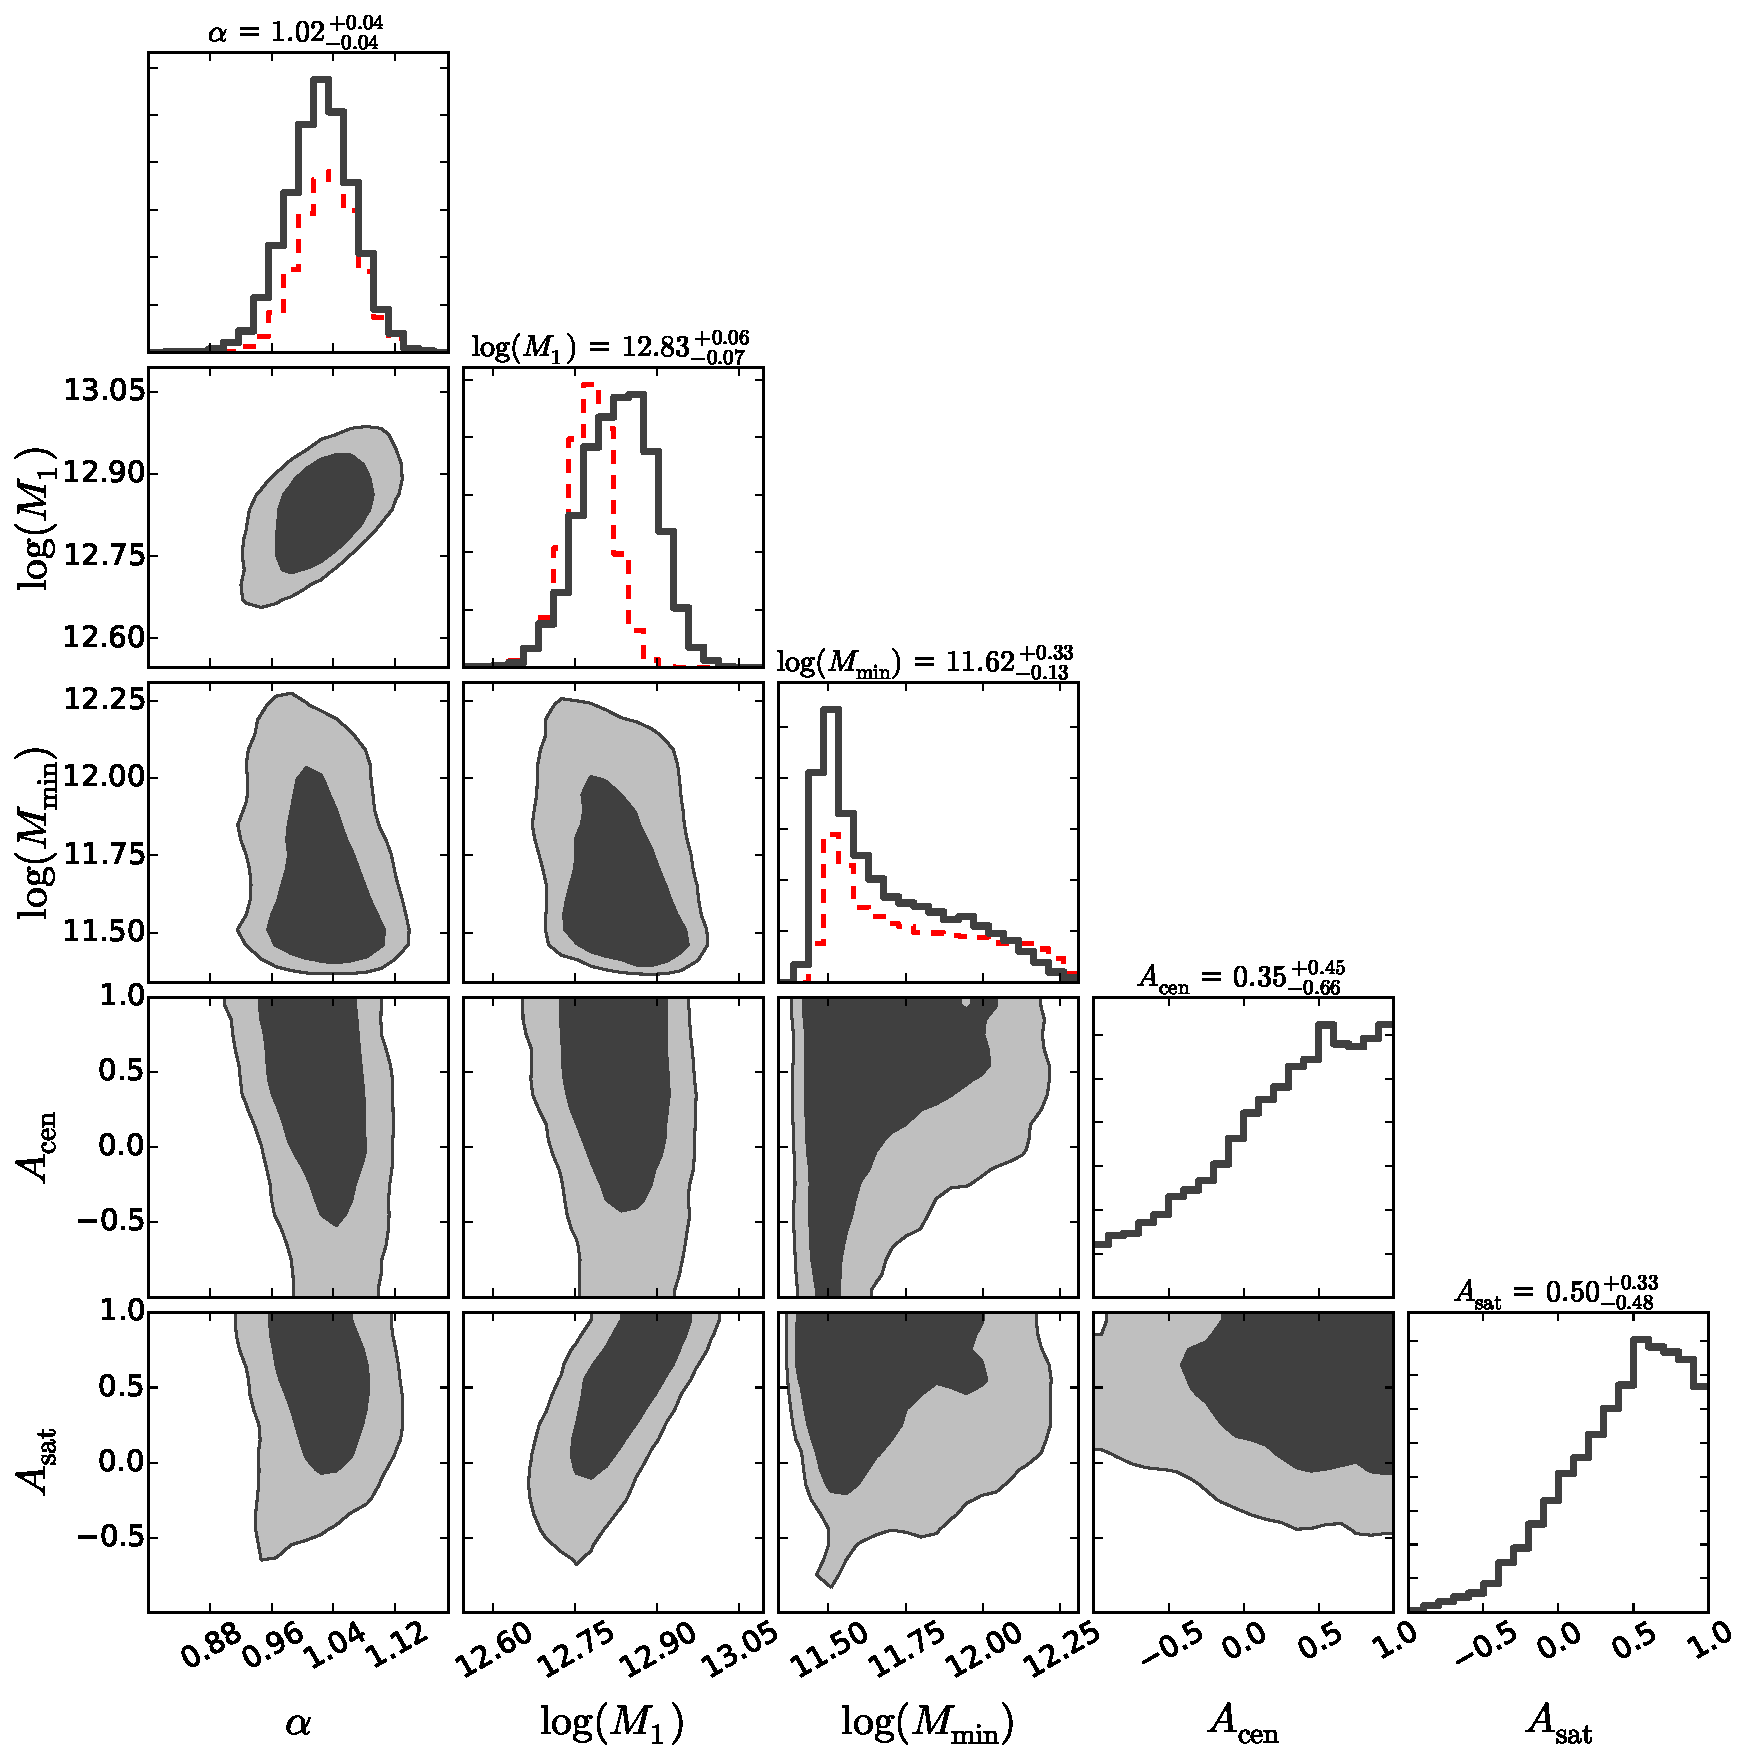
\includegraphics[width=15.0cm]{Mr19ABTri.pdf}
\caption{ Two-dimensional marginalized constraints on decorated HOD
  parameters inferred from fits to $\wprp(\rp)$ data for the $M_r<-19$
  sample. The contours and histograms along the diagonal panels are as
  in Fig.~\ref{fig:Mr20triangle}. The decorated HOD models include a
  two-parameter model for assembly bias. The HOD parameter $\log
  (M_0)$ is extremely poorly constrained by the data and has been
  suppressed for clarity. Likewise, as in Fig.~\ref{fig:Mr20triangle},
  $\sigma_{\log M}$ and $\log (M_{\rm min})$ share a narrow
  degeneracy, so we have suppressed $\sigma_{\log M}$ in order to make
  constraints on other parameters more easily visible.  }
\label{fig:Mr19ABtriangle}
\end{center}
\end{figure*}
%----------------------------------------------------------------------------------------------


%---------------------------------------------------------------------------------------------------
\begin{figure*}
\begin{center}
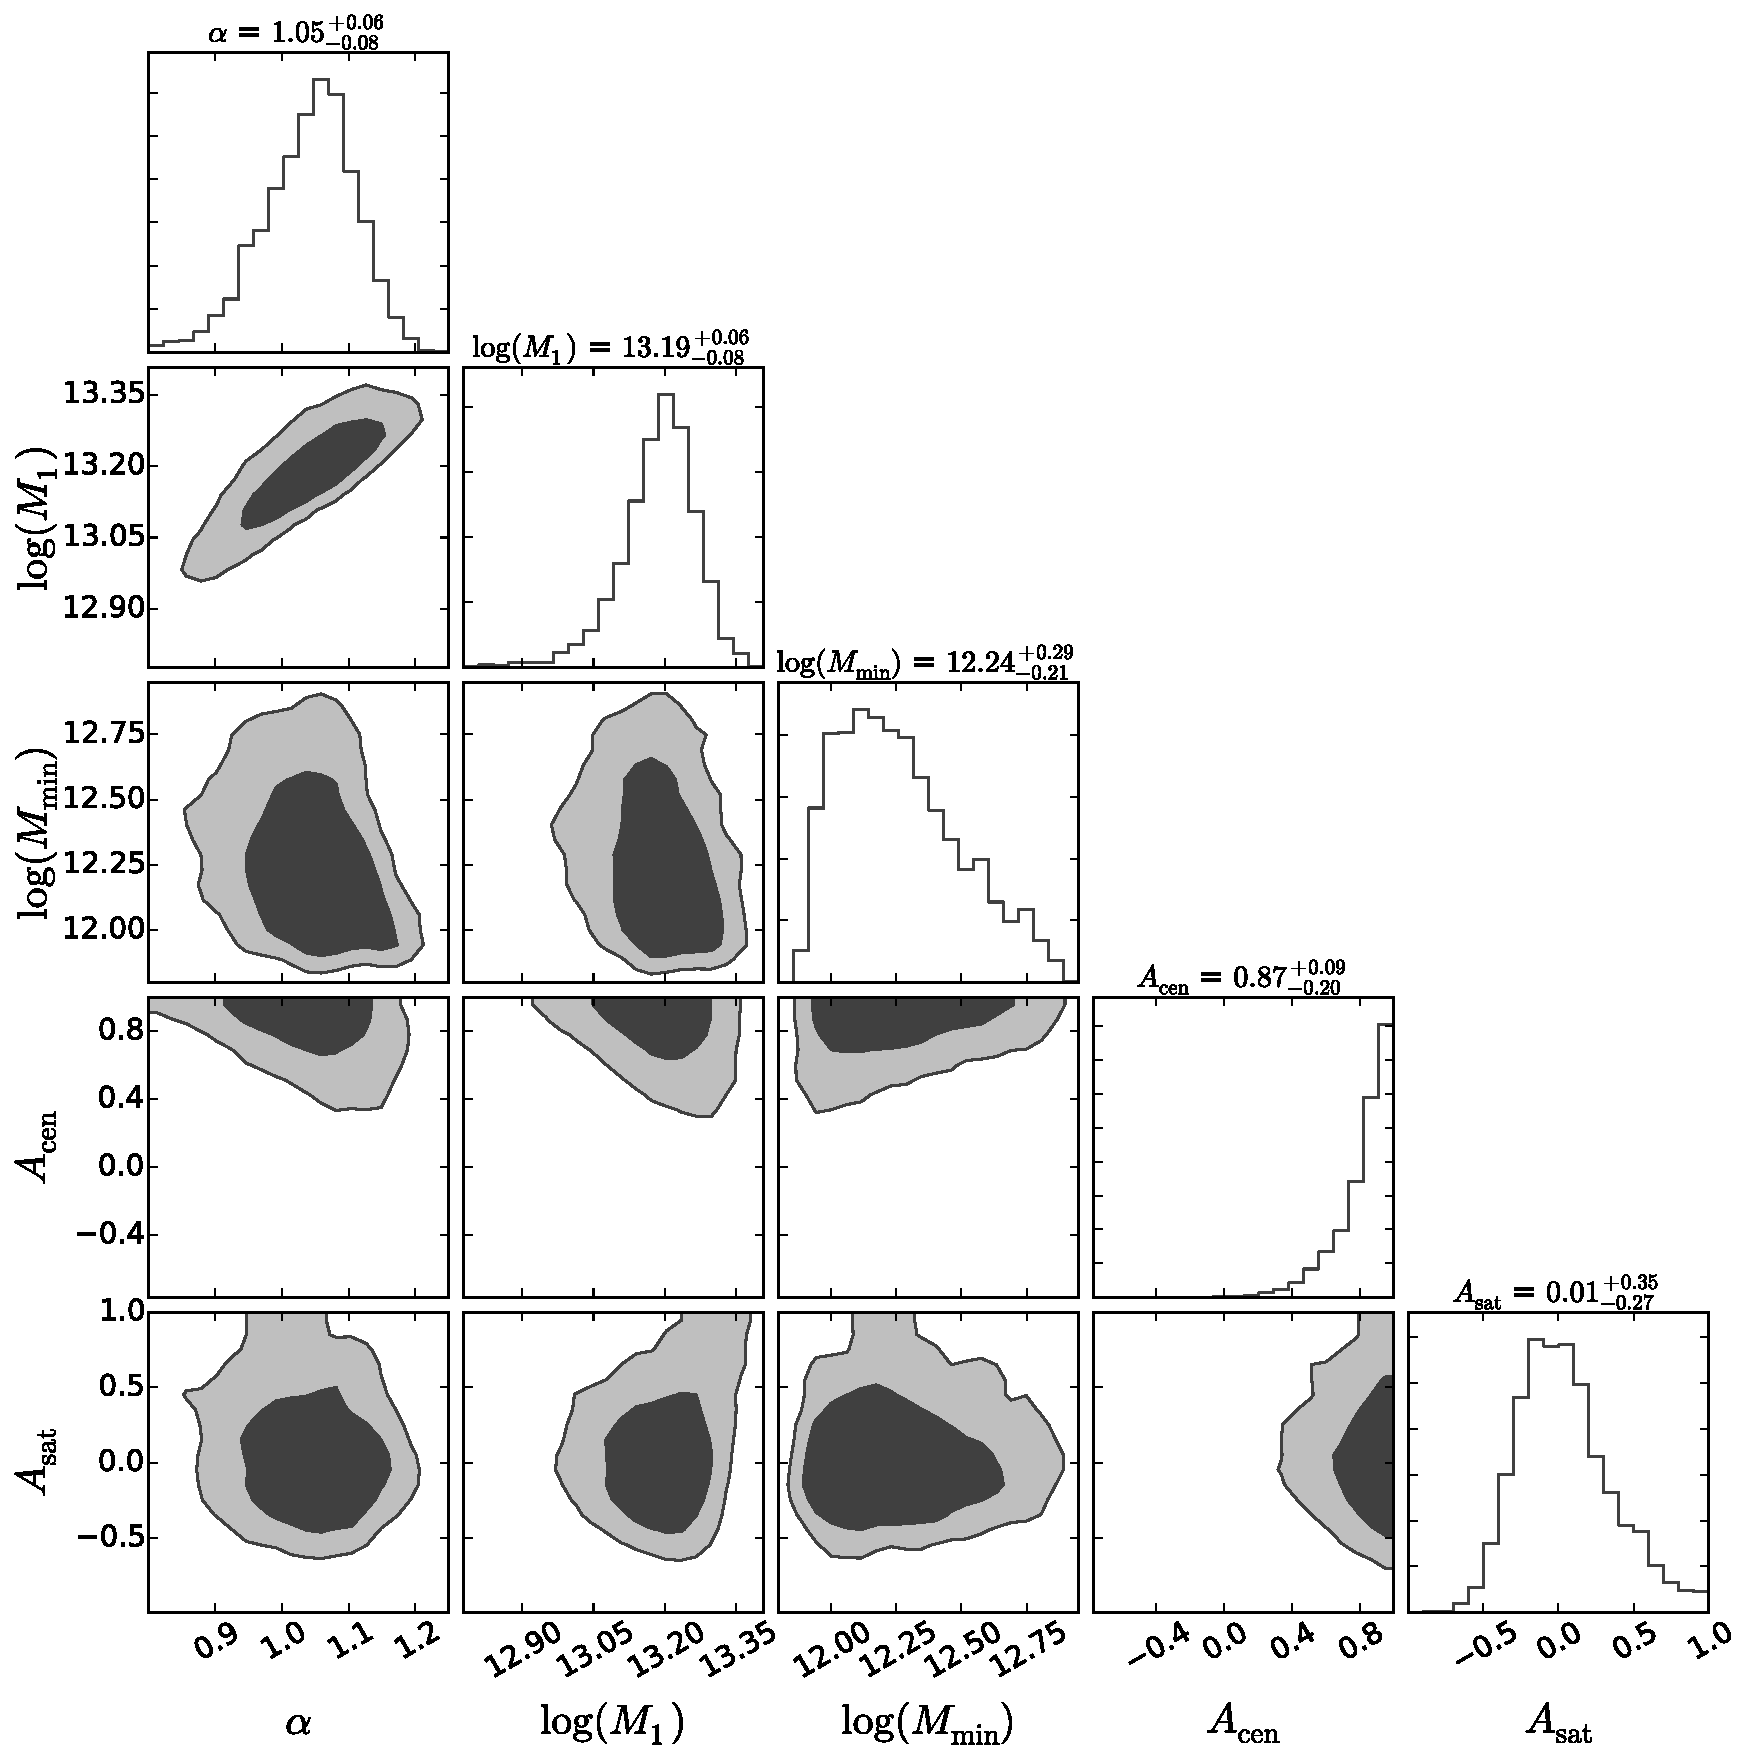
\includegraphics[width=15.0cm]{Mr20ABTri.pdf}
\caption{
The same as Figure~\ref{fig:Mr19ABtriangle}, but for the $M_r<-20$ sample.
}
\label{fig:Mr20ABtriangle}
\end{center}
\end{figure*}
%---------------------------------------------------------------------------------------------------

%=-------------------------------------------------------------------------------------------------
\begin{figure*}
\begin{center}
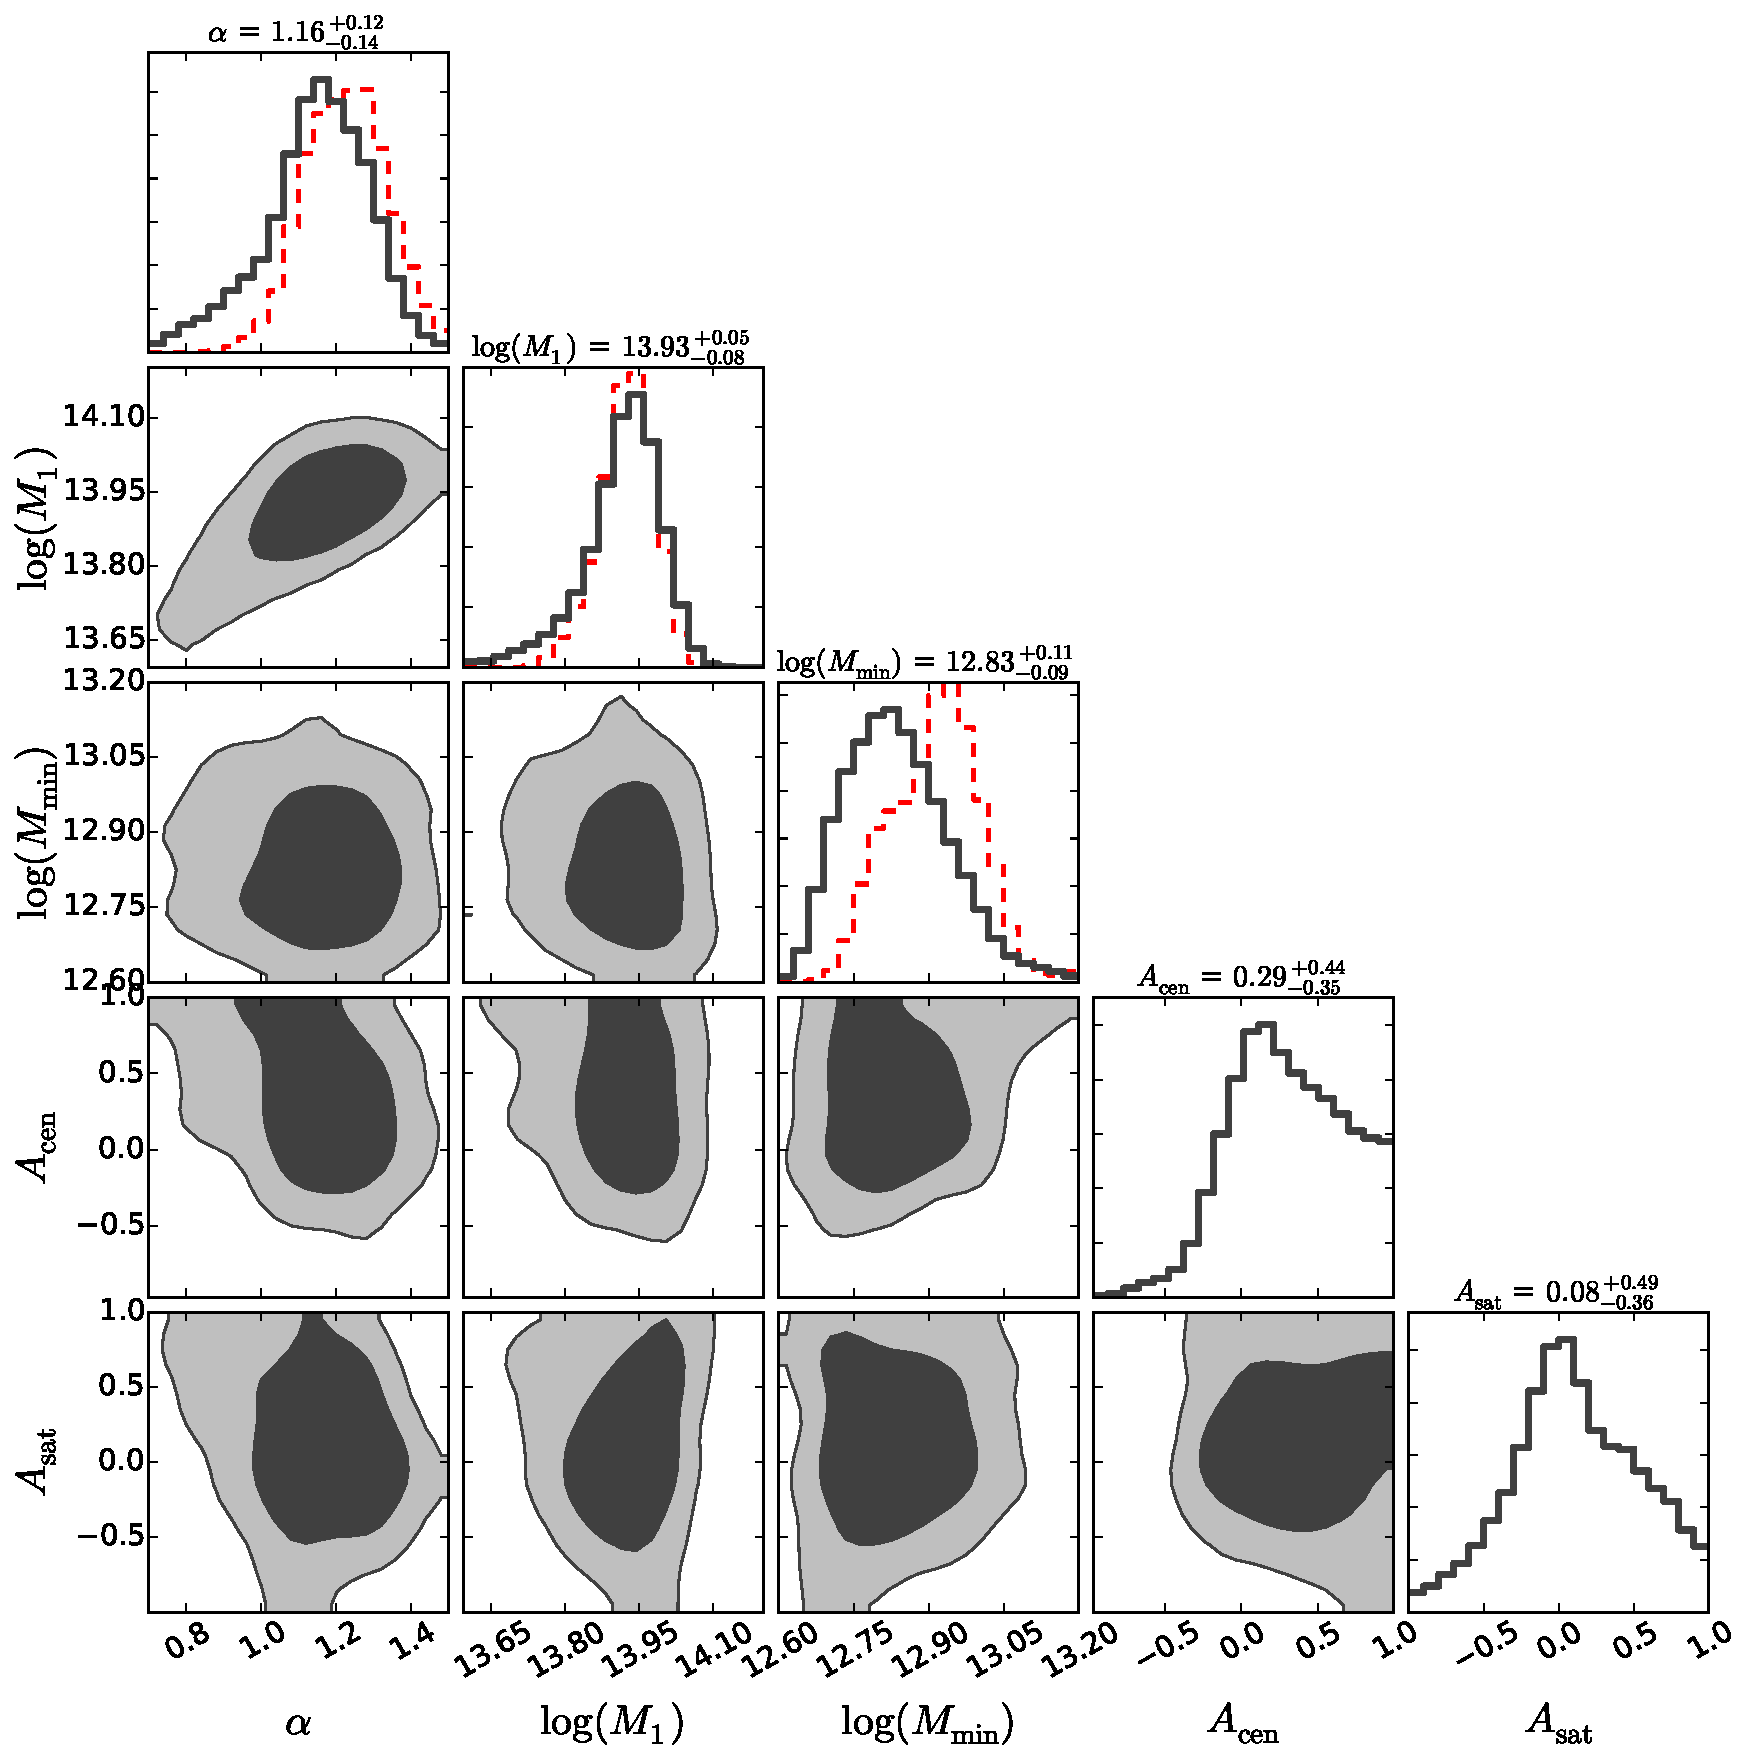
\includegraphics[width=15.0cm]{Mr21ABTri.pdf}
\caption{
The same as Figure~\ref{fig:Mr19ABtriangle}, but for the $M_r<-21$ sample.
}
\label{fig:Mr21ABtriangle}
\end{center}
\end{figure*}
%----------------------------------------------------------------------------------------------------


Table~\ref{table:parameters} and Figures~\ref{fig:Mr19ABtriangle}-\ref{fig:Mr21triangle} 
all make several simple, generic points. Introducing additional parameter 
freedom associated with galaxy assembly bias generally increases the viable parameter 
space, even for the subset of standard HOD parameters. Constraints on the 
standard HOD parameters are generally less restrictive. This is exactly what is 
expected from the introduction of additional parameter freedom. 


Focusing attention on the parameters describing galaxy assembly bias, it is 
evident that these parameters are often quite poorly constrained by galaxy 
clustering data. This is important as it implies that galaxy clustering of the precision 
of SDSS DR7 measurements cannot rule out, or strongly restrict galaxy assembly 
bias in many cases. Nonetheless, it is apparent that the presence of assembly bias 
can alter the inferred HOD, or more generally, the inferred relationship between 
galaxies and halo mass. This is most evident for the $M_r < -20$ threshold sample, 
for which there are significant differences in the inferred values of all baseline HOD 
parameters between models with and without galaxy assembly bias. Other threshold 
samples exhibit significant changes particularly for $\alpha$, and to a lesser degree 
for $\log (M_{\rm min})$ and $\sigma_{\log M}$. 


Beyond those generic conclusions, a few specific cases are worthy of further examination. 
Consider the $M_r < -20$ sample. The inferred value of $A_{\rm cen} > 0.28$ at 99\% 
confidence. In this case the data strongly prefer $A_{\rm cen} > 0$ and thus strongly prefer 
galaxies to reside in halos of larger concentration at fixed halo mass. This particular threshold 
sample is the most significant outlier in this regard. Nevertheless, there are hints of assembly 
bias in other samples. Satellite galaxies show a marginal preference for occupying halos of 
higher concentration in the $M_r < -19$ threshold sample. The $M_r < -19$ sample exhibits 
weak preference for a positive correlation of galaxy occupation with halo concentration at fixed 
mass for both satellite galaxies and central galaxies. Continuing upward with luminosity, 
the $M_r < -20.5$ sample exhibits a significant preference for central galaxy assembly bias. 
Lastly, there is no preference for either central galaxy or satellite galaxy assembly bias 
for the $M_r < -21$ threshold sample, for which both $A_{\mathrm{cen}}$ and $A_{\mathrm{sat}}$ 
are consistent with zero will within 1$\sigma$. These data suggest that assembly bias 
may be present in the real universe.


%-------------------------------------------------------------------------------------------------------------------------------------------------
\begin{table}
\begin{center}
{\renewcommand{\arraystretch}{1.3}
\renewcommand{\tabcolsep}{0.2cm}
\begin{tabular}{c c}
\hline 
\hline
$M_r$ Threshold & $\Delta \mathrm{BIC}$ \\ 
\hline
-21 & -0.54 \\
-20.5 & 1.33 \\
-20 & 4.56\\
-19.5 & 0.26\\
-19 & 4.37\\
\hline
\end{tabular}
\medskip
\caption{
Change to the Bayesian Information Criterion, $\Delta \mathrm{BIC}$, 
after introducing additional parametric freedom to accommodate galaxy 
assembly bias. Sign convention is such that positive values favor models including 
assembly bias, negative values favor standard HOD models with no assembly bias parameters. Changes in 
the Bayesian Information Criterion $\vert \Delta \mathrm{BIC}\vert \ge 5$ strongly favor one model 
over another.
}
 }
 \label{table:priors}
 \end{center}
\end{table}
%--------------------------------------------------------------------------------------------------------------------------------

%------------------------------------------------
\section{Conclusions}
\label{section:conclusions}
%------------------------------------------------

We have re-analyzed the SDSS DR7 measurements of projected galaxy clustering,  $\wprp,$ and number density, $n_{\rm g},$ originally published in \citet{zehavi_etal11}. Our work is especially novel in that we provide the first quantitative constraints on assembly bias derived from the Decorated HOD, an extension to the traditional HOD introduced in \citet{hearin_etal16} developed for exactly this purpose. 
We enumerate our most important conclusions below. 
\ben
\item It is not possible to rule out galaxy assembly bias using SDSS DR7 measurements of $\wprp$ and $n_{\rm g}.$
\item Decorated HOD fits to $\wprp$ and $n_{\rm g}$ favor significant levels of assembly bias, particularly in the lower luminosity thresholds we study. Both the $\magr<-20, -20.5$ samples prefer relatively strong central galaxy assembly bias, while at lower luminosities, the $\magr<-19$ sample favors satellite assembly bias. 
\item Galaxy assembly bias generally weakens for brighter galaxy samples: Decorated HOD fits to the $\magr<-21$ sample are consistent with both $\abias^{\rm cens}=0$ and $\abias^{\rm sats}=0.$ This consistent with the well-established result that {\em halo assembly bias} weakens with increasing halo mass over the dynamic range relevant to these galaxy samples \citep[see, e.g., Figure 8 of][and references therein]{hearin_etal16}. 
\item Our posteriors and best-fit parameters summarized in Table \ref{table:parameters} supersede the values published in \citet{zehavi_etal11}, as direct-mock-population together with the Decorated HOD allows us to account for highly significant systematics that have heretofore been neglected from all HOD fits to SDSS data. We note that our findings update the original \citet{zehavi_etal11} results {\em even for our fits in which assembly bias has been fixed to zero}, since the original results derive from unconverged MCMC chains that do not sufficiently sample the HOD model posteriors. 
\een
We conclude by noting that since $\wprp$ and $n_{\rm g}$ are already very well-measured in DR7, it is likely that further improvements on assembly bias constraints at low-redshift will require additional observational measurements, e.g., galaxy--galaxy lensing, group statistics, etc.

%------------------------------------------------
\section{Acknowledgements}
\label{section:acknowledgements}
%------------------------------------------------

The authors gratefully acknowledge the Gauss Centre for Supercomputing
e.V. (www.gauss-centre.eu) and the Partnership for Advanced
Supercomputing in Europe (PRACE, www.prace-ri.eu) for funding the
MultiDark simulation project by providing computing time on the GCS
Supercomputer SuperMUC at Leibniz Supercomputing Centre (LRZ,
www.lrz.de). The Bolshoi simulations have been performed within the
Bolshoi project of the University of California High-Performance
AstroComputing Center (UC-HiPACC) and were run at the NASA Ames
Research Center. FvdB is supported by the US National Science
Foundation through grant AST 1516962. {\bf AZ; add yours as well.}



%------------------------------------------------
\bibliography{ms.bib}

%------------------------------------------------
\end{document}
%------------------------------------------------
